\chapter{Image reconstruction as an auxiliary task for generative modeling}
\label{chap:chapter2}
\graphicspath{{images/chapter2/}, {tikz/chapter2/} }

\begin{chapterabstract}
		While the  Conditional GAN approach \citep{Mirza2014} is theoretically generic enough to model any kind of conditioning, it lacks some form of control or guarantee on the respect of these constraints. In this chapter, we propose to explore another approach for conditioning a GAN model through an image reconstruction task, which consists in (re-)generating images from a very sparse set of randomly-positioned pixels known beforehand. This is directly motivated by applications in geosciences, most notably the generation of subsurface rock structure \citep{Laloy2019,Ruffino2017}.  We reformulate this conditional generation task as a Maximum A Posteriori estimation and find a solution in the form of an explicit auxiliary reconstruction task, which adds to the original unconditional GAN objective as an additional loss term. Complemented with the PacGAN \citep{Lin2018} variant for training GANs, this approach enables the generation of diverse samples from a sparse pixel map. As opposed to the more classical Conditional GAN approach, this auxiliary task is interpretable and a hyperparameter allows to control the importance of the conditioning in the learning process. We evaluate our approach on the classical MNIST, FashionMNIST and CIFAR10 datasets, as well as a custom-made texture dataset. Finally,  we apply this approach to a to a dataset of subsurface rock formations.
\end{chapterabstract}\\



The work in this chapter has led to the publication of the following papers: 
\begin{itemize}
	\item Cyprien Ruffino, Romain H\'erault, Eric Laloy and Gilles Gasso (Nov. 2019). Pixel-Wise Conditioning of Generative Adversarial Networks.
 In:  Proceedings of the 27th European Symposium on Artificial Neural Networks (ESANN).
	\item Cyprien Ruffino,  Romain H\'erault, Eric Laloy and Gilles Gasso (Apr. 2020). Pixel-Wise Conditioned Generative Adversarial Networks for Image Synthesis and
Completion. In: Neurocomputing. 
\end{itemize}

\newpage
\minitoc

\section{Introduction}

As we have seen in \citesec{subs:CGAN}, Conditional GANs enables a variety of conditioned generation, such as class-conditioned image generation \citep{Mirza2014}, image-to-image translation \citep{Isola2016, Wang2018}, image super-resolution \citep{Wang2020} or image inpainting \citep{Pathak2016}. While this approach, combined with enough data and the right network architectures, has led to spectacular results \citep{Karras2020}, it lacks some mechanism to strongly enforce the respect of the constraints. Indeed, it only rely on the adversarial learning process with no explicit method for including the constraints into the generation task.

In this chapter,  we propose to study in depth the less general problem of reconstructing images from very few pixels (usually less than a percent). We refer to these conditioning pixels as a constraint map $y$. This kind of task has several direct applications, in which recovering the entirety of a signal with very sparse measurements is necessary, for example in domains where measuring the signal is expensive. Here, we study the task of recreating a subsurface rock formation from very few measurements, which has direct applications in geology. This is motivated by previous works on subsurface data generation \citep{Laloy2018, Laloy2019}.

To reconstruct the missing information, a generative  model must able to generate high quality images coherent with the given pixel values by leveraging on a training set of similar images. The model aims to match the distribution of the real images conditioned on a highly scarce constraint map. While the \ac{CGAN} approach is theoretically capable of tackling this problem, there is in practice no guarantee that the constraints will be enforced in the generated image. In settings where respecting these constraints is crucial, this is a significant limitation.

To explicitly push the generated images towards honoring the prescribed pixel values, we propose to use a reconstruction loss measuring how close real constrained pixels are to their generated counterparts.  By re-framing this problem as a Maximum A Posteriori estimation, we show that minimizing this loss is equivalent to maximizing the log-likelihood of the constraints given the generated image. Thereon we derive an objective function by adding a reconstruction loss to the adversarial loss of \ac{GAN}. This introduces a hyperparameter in the objective function.

 We analyze the influence of this hyperparameter in terms of quality of generated images and the respect of the constraints. Specifically, empirical evaluation on FashionMNIST~\citep{Xiao2017} evidences that the regularization parameter allows for controlling the trade-off between samples quality and constraints fulfillment. 
Additionally to show the effectiveness of our approach, we conduct experiments on CIFAR10 \citep{Krizhevsky2009}, CelebA \citep{Liu2015} or texture \citep{Jetchev2017} datasets using various deep architectures including fully convolutional network. We also evaluate our method on a classical geological problem which consists of generating 2D geological images of which the spatial patterns are consistent with those found in a conceptual image of a binary fluvial aquifer\citep{Strebelle2002}\citep{Laloy2018}. Empirical findings reveal that the used architectures may lack stochasticity in the generated samples, that is the GAN input is often mapped to the same output image irrespective of the variations in latent code \citep{Yang2019}. We address this issue by resorting to the PacGAN \citep{Lin2018} strategy, that consists in providing pairs of samples to the discriminator for either the generated images and the images from the dataset.

As a conclusion, our approach performs well both in terms of visual quality and respect of the pixel constraints while keeping diversity among generated samples. Evaluations on CIFAR-10 and CelebA show that the proposed generative model always outperforms the CGAN approach on the respect of the constraints and either come close or outperforms it on the visual quality of the generated samples.

The remainder of the chapter is organized as follows. In Section \ref{sec:related_work}, we review the relevant related  work focusing first on two families of methods for dealing with image reconstruction from highly altered training samples, optimization-based approaches and conditional generation-based ones. Section \ref{sec:bridging} propose to review the links between these two categories of approaches, introduces our approach for image reconstruction and propose some theoretical insight to justify it. In Section \ref{sec:experiments_protocol}, we present the experimental protocol and evaluation measures while Section \ref{subs:results} gathers quantitative and qualitative effectiveness of our approach. The last section concludes the paper.

The contributions of this chapter are summarized as follows:
\begin{itemize}[nosep]
	\item We propose a method for learning to generate images with a few pixel-wise constraints.
	\item We expose a controllable trade-off between the image quality and the constraints' fulfillment.
	\item We showcase a lack of diversity in generating high-dimensional images which we solve by using  PacGAN\citep{Lin2018} technique. Several experiments allow to conclude that the proposed formulation can effectively generate diverse and high visual quality images while satisfying the pixel-wise constraints. 
\end{itemize}

\section{Approaches for image reconstruction}
\label{sec:related_work}

Image reconstruction is the task of retrieving an image from a very altered source, which can take several forms from additive noise to missing parts of the image. In this chapter, we study a rather extreme case of alteration, which is the removal of over 99\% of the original image, leaving only a handful of pixels scattered at random positions.

In this section, we propose an overview of this problem and some of the seminal approaches for solving similar tasks. We expose two families of methods: per-sample optimization and conditional modeling, and detail some strengths and weaknesses for both of these families.

\subsection{The problem of image reconstruction}
\label{sub:image_reconstruction_problem}

Image reconstruction belong to a family of problems consisting in retrieving an image from an altered one. Among this family are problems such as in inpainting \citep{Bertalmio2000} (Figure \ref{fig:inpainting}) or image denoising  \citep{Goyal2020} which consists in retrieving altered or missing parts of an image \citefig{fig:image_completion_task}. It however differs in that since most of the original image is unavailable, an image reconstruction approach cannot simply retrieve missing parts of a semantically rich image, but instead needs to generate a new image, leveraging on a prior such as generative modeling, while ensuring that the resulting image is coherent with the values given as input.

Before delving into the details, let introduce the notations related to the problem. We denote by $X \in \setX$ a random variable and $\vx$ its realization. Let $\p{\mx}$ be the distribution of $\mx$ over $\setX$ and $\p{\mx}$ be its evaluation at $x$. Similarly $\p{\mx|\my}$ represents the distribution of $\mx$ conditioned on the random variable $\my \in \setY$. 

 Assume $\vy$ is the given set of constrained pixel values. To ease the presentation, let consider $\vy$ as a $n\times p\times c$ image with only a few available pixels (less than $1\%$ of $n\times p\times c$). We will also encode the spatial location of these pixels using a corresponding binary mask $M(\vy) \in \{0,1 \}^{n\times p\times c}$. 

Given a set of images $\vx \in \setX = [-1, 1]^{n\times p\times c}$  (see Figure \ref{fig:digit}) drawn from an unknown distribution $\p{\mx}$ and a sparse matrix  $\vy \in  \setY = [-1, 1]^{n\times p\times c}$ (Figure \ref{fig:pixelwise_gen}) as the given constrained pixels, the problem consists in finding an image $\Hat{\vx}$ that maximizes $\p{\Hat{\vx}}$ while satisfying the constraints $\vy$.

In other words, the problem consists in retrieving $\vx$ such that $\vy = M(\vy) \odot \vx$ and $\vx$ is close to the data distribution. More formally, we can formulate it as 

\begin{equation}
	\label{eq:formulation_ur_primary_GAN}
	\vx^* = \arg\max_\vx \p{\vx} \enspace \text{subject to} \enspace \vy = M(\vy) \odot \vx \nonumber
\end{equation}

\noindent where $\odot$ stands for the Hadamard (or point-wise) product and $M(\vy)$ for the mask, the sparse matrix with entries equal to one at constrained pixels location. Note that this expression can also be formulated with a matrix product, since \\ $\vect(M(\vy)\odot \vx) = \text{Tr}(\text{Diag}(\vect(M(\vy)))\vect(\vx))$.

\begin{figure}[t]
	\centering
	\begin{subfigure}[t]{0.33\textwidth}
		\centering
		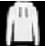
\includegraphics[width=3cm]{fashion_sample.jpg}
		\caption{Original \\ Image}
		\label{fig:digit}
	\end{subfigure}\begin{subfigure}[t]{0.33\textwidth}
		\centering
		
\includegraphics[width=3cm]{fashion_sample_inpainting.jpg}
		\caption{Inpainting\\Input}
		\label{fig:inpainting}
	\end{subfigure}\begin{subfigure}[t]{0.33\textwidth}
		\centering
		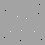
\includegraphics[width=3cm]{fashion_sample_pixel.jpg}
		\caption{Constraint\\Map}
		\label{fig:pixelwise_gen}
	\end{subfigure}
	\caption[Inpainting and image reconstruction]{Difference between regular inpainting (\ref{fig:inpainting}) and the problem undertaken in this work (\ref{fig:pixelwise_gen}) on a real sample (\ref{fig:digit}).}
	\label{fig:image_completion_task}
\end{figure}


\subsection{Image reconstruction with optimization}

A first approach to tackle the image reconstruction process is to directly trying to recover the image through optimization. As such, we can consider the image reconstruction problem as recovering a signal that has been altered. Thus, the problem can be formulated as a system of the form

\begin{equation}
		\label{eq:reconstruction_system}
		\vy = A\vx + \epsilon \enspace,
\end{equation}
where  $A \in \mathbb{R}^{n\times m}$ is a wide ($n \ll m$), matrix (so called ``measurement matrix'') and $\epsilon$ is noise. Although the system is linear, it is highly under determined, thus solving it generally is impossible. However, by including prior knowledge on the signal $\vx$ and by ensuring some constraints on the matrix $A$, solving this system can be done using optimization or linear programming.

Most notably, \citet{Candes2005} introduced \textbf{Compressed Sensing}, which consists in solving the system by assuming that the signal $\vx$ is sparse. In order to guarantee that the obtained image is indeed a reconstruction, they introduced the the Restricted Isometry Property (\ac{RIP}) \citep{Candes2008} on the family of matrices $A$, which states that for two samples $x_1,x_2 \sim \p{X}$, 
%
\begin{equation}	
	\label{eq:rip}
	(1 - \alpha)||x_1 - x_2||_2^2 \leq ||A(x_1 - x_2)||_2^2 \leq (1 + \alpha) ||x_1 - x_2||_2^2 \enspace,
\end{equation}

where $\alpha$ is a small constant. This states that distances between two samples are conserved when altered by $A$. Solving this problem can be done with linear programming as 
%
\begin{equation}
	\label{eq:compressed_sensing}
	\Hat{\vx} = \arg\min_\vx  ||\vx||_1 \enspace \text{subject to} \enspace A\vx = \vy \enspace .
\end{equation}
%
This method bears three important issues, the first one being that, in practice, the assumption of sparsity on $\vx$ is usually not enforced, especially when the measurement process is noisy. This requirement can be replaced by the more generic approach of considering sparsity in another basis. Let  $B$ be a basis such that for $\vx = B\vs$, the majority of the coefficients of $\vs$ are zero. Thus, the problem becomes 
%
\begin{align}
	\label{eq:compressed_sensing_basis}
	\Hat{\vs} = \arg\min_\vs  ||B\vs||_1 \enspace &\text{subject to} \enspace AB\vs = \vy \enspace ,\nonumber\\
	\Hat{\vx} &= B\Hat{\vs} \enspace .
\end{align}
%
By either carefully selecting $B$, such as a Fourier or wavelet basis\citep{Parkale2016}, or learning it with, for example, sparse dictionary \citep{Chen2016b} or basis pursuit \citep{Shaobing1994, Donoho2006}, this approach is much more robust and provides good results in real-world situations \citep{Kolev2011, Duarte2008}.

The second problem of this approach is that it requires to solve an optimization problem for each sample. Even if the compressed sensing approach allows for the problem to be formulated as linear programming, which can be solved in polynomial time,  it is still computationally expensive. Finally, the third issue is that the measurement matrix $A$ does not necessarily respect the \ac{RIP}. As we have seen, the \ac{RIP} guarantees the coherency of the reconstructed sample. However, verifying that the matrix $A$ respects the \ac{RIP} is NP-hard in general. While several approaches for image compression uses techniques for generating random matrices that have a high probability of respecting the \ac{RIP} \citep{Rudelson2008,Rauhut2010}, there are no guarantees in the case when $A$ is fixed, such as image reconstruction.

\subsection{Conditional generation for image reconstruction}

As opposed to the aforementioned methods that rely on directly finding the best solution to revert the alteration process through optimization, methods based on conditional generation try to learn the conditional distribution $\p{X|Y}$ and either aims to generate the most probable solution or provide a sampling mechanism over potential solutions. 

In the case of image reconstruction, a generative model $\G$ which input is constraint map $y \in  [-1, 1]^{n\times p\times c}$ learns to generate an image satisfying the constraints while likely following the distribution $\p{X}$ (see \citefig{fig:image_completion}). For a generative model to provide a sampling mechanism, the common solution consists in using a random vector $\vz$  sampled from a known distribution $\p{Z}$ (usually uniform or  Gaussian) over a space $\setZ$ that will be used as a latent variable for the model.

Although \ac{CGAN} was initially designed for class-conditioned image generation by setting $\vy$ as the class label of the image, it can naturally be applied to several types of conditioning information, including constraint maps, thus obtaining an  image reconstruction with a high likelihood on the conditional distribution $\p{X|Y}$ is equivalent on taking a sample on the distribution of the generative model $\G$
%
\begin{align}
	\label{eq:CGAN_problem_reco}
	\G^* = \arg\min_\G\max_\D &\esp{\vx,\vy\sim \p{X,Y}} [\log \D(\vx, \vy)] +  \esp{\vy\sim \p{Y} \\ z\sim\p{Z}} [1 - \log \D(\G(\vy, \vz), \vy)] \enspace , \nonumber \\
	\Hat{\vx} &= \G^*(\vy, \vz), \enspace \text{with} \enspace \vz \sim \p{Z}
\end{align}
%
where $\vy$ is the constraint map and $\D$ is the discriminator network.
\CR{TODO}
However, CGAN-based inpainting methods rely on generating a patch that will fill up a structured missing part of the image and achieve impressive results. Thus, they are not well suited to reconstruct very sparse and unstructured signal \citep{Demir2018}. 

The most common approach os 
\CR{Transition}

Another of these approaches is \textbf{Ambient \ac{GAN}} \citep{Bora2018} (Figure \ref{fig:ambientgan}), which aims at training an unconditional generative model using a dataset of noisy or incomplete samples $\setY$. Ambient \ac{GAN} attempts to produce unaltered images $\tilde{\vx}$ which distribution matches the true one without accessing to the original images $\vx$. For the sake, Ambient \ac{GAN} considers lossy measurements such as blurred images, images with removed patch or removed pixels at random (up to 95\%), leading to sparse pixel map $\vy$. This lossy measurement is simulated with a function $f_\theta$ instead of the matrix $A$, whose parameter $\theta$ indicates the pixels to be removed, such that

\begin{equation}
	\label{eq:denoising_system}
	\vy = f_\theta(\vx) \enspace.
\end{equation}

The underlying optimization problem solved by AmbientGAN is therefore stated as

\begin{equation}
	\label{eq:ambientgan}
	\min_G \max_D L(D, G) = \mathop{\mathbb{E}}_{\substack{y\sim \p{Y}}} \Big[\log(D(y))\Big] + \mathop{\mathbb{E}}_{\substack{z\sim \p{Z} \\\theta \sim p_\theta}} \Big[ \log(1-D(f_\theta(G(z))))\Big] \enspace.
\end{equation}

\textbf{Unsupervised Image Reconstruction} \citep{Pajot2019} \CR{Détailler plus? Refaire} combines the AmbientGAN approach with an additional reconstruction task that consists in reconstructing the $f_\theta(G(y))$ from the twice-altered image $\tilde{y} = f_\theta(G(y))$ and $\hat{y} = f_\theta(G(f_\theta(G(y))))$,

\begin{equation}
	\label{eq:unir}
	\min_G \max_D L(D, G) = \mathop{\mathbb{E}}_{\substack{y\sim \p{Y}}} \Big[\log(D(y))\Big] + \mathop{\mathbb{E}}_{\substack{y\sim \p{Y}}} \Big[ \log(1-D(\hat{y}))\Big] + ||\hat{y} - \tilde{y} ||^2_2 \enspace.
\end{equation}
\noindent
The $\ell_2$ norm term ensures that the generator is able to learn to revert $f_\theta$ i.e. to revert the alteration process on a given sample. This  allows the reconstruction of realistic image only from a given constraint map $y$. However the reconstruction process is deterministic and does not provide a sampling mechanism.



\section{Bridging conditional generation and optimization-based reconstruction}
\label{sec:bridging}

 As we have seen, two main categories of solution aim to tackle the problem of image reconstruction. First, the approaches that try to directly solve the problem by finding a solution through optimization, among them is compressed sensing. However, the main drawback of these families of approaches are that they require to solve an optimization problem for each reconstructed image, which is a heavy computational burden. 

Then, the approaches that aims to learn the conditional data distribution $\p{X|Y}$ and try to reconstruct the image by sampling on this distribution. Among these approaches are \ac{CGAN}-based methods, norm-based methods, AmbientGAN or UNIR. While they have the advantage of not requiring to solve an optimization problem for each sample, they cannot guarantee that the constraints will be respected.

In this section, we study two ways of linking these families of approaches. First, by optimizing in the latent space of a generative model. This allows to overcome the explicit assumptions that have to be made, such as sparsity, by using said generative model as a prior on the real data distribution. The second approach consists in re-framing the reconstruction problem as a maximum a posteriori estimation. We find that by exploiting the formulation of the conditional distribution learning problem, replacing the implicit conditioning of the \ac{CGAN} by a norm-based reconstruction loss is an approach that naturally emerges from the denoising formulation \citeq{eq:denoising_system}, thus providing a rationale for the use of these losses in similar approaches.

While the first category of these approaches conserves the issue of the computation time due to the optimization process that is required in order to reconstruct an image, the second one allows for the training a generative model to directly sample potential solutions to the image reconstruction problem without solving an optimization problem for each sample. It also naturally provides a mechanism for controlling the trade-off between the respect of the constraints and the likelihood of the reconstructed image.

\subsection{Generative modeling as a prior for optimization}

While optimization-based methods for image reconstruction have the advantage of explicitly modeling the constraints, which ensures that they will be enforced in the reconstructed image, there are no guarantees on the quality of the reconstruction process if the \ac{RIP} \citeq{eq:rip} is not respected in the measurement matrix $A$. In the case of the image reconstruction process, this means that while the reconstructed image $\hat{\vx}$ is guaranteed to enforce the constraints, it is not necessarily close to the real data distribution $\p{\vx}$.

\textbf{Compressed Sensing with Meta-Learning} \citep{Wu2019} extend compressed sensing by replacing the sparsity assumption on the signal $\vx$ a learned prior on the data distribution $\p{X}$, as a generative model $\G$.  By first generating an image $\G(\vz)$ and exploring the latent space $\setZ$ of the generative model $\G$ by minimizing $||A\G(\vz) - \vy||^2_2$, so that altering the generated image gives $\Hat{\vy}=A\G(\vz)$ where $\Hat{\vy}$ is as close as possible to $\vy$. Then, Compressed sensing with meta-learning trains the generative model $\G$ to enforce the \ac{RIP} (\citeq{eq:rip}) so that it does not try to map all $\G(\vz)$ into the null space of $A$. The overall problem induced by this approach is formulated as

% 		\begin{multline}
% 	    	\min_G L(G) = \mathop{\mathbb{E}}_{\substack{x\sim \p{X}\\y\sim \p{Y}\\z\sim \p{Z}}} \Big[\Big( (||f_\theta (x - G(z))||_2^2 - ||x - G(z)||_2^2)^2 + (||f_\theta (x - G(\hat{z}))||_2^2 - ||x - G(\hat{z})||_2^2)^2 \\
% 	    	+ (||f_\theta (G(z) - G(\hat{z}))||_2^2 - ||G(z) - G(\hat{z})||_2^2)^2 \Big) / 3
% 	    	+ ||y - f_\theta(G(\hat{z})) ||^2_2\Big]\\
% 	    	\text{where } \hat{z} = \min_z ||y - f_\theta(G(z)) ||^2\enspace.
% 		\end{multline}

\begin{multline}
	\label{eq:csmeta}
	\min_\G L(\G) = \mathop{\mathbb{E}}_{\substack{\vx\sim \p{X}\\\vy\sim \p{Y}\\\vz\sim \p{Z}}} \Big( \sum_{\substack{\vx_1, \vx_2 \in \setS\\x_1 \ne \vx_2}}((||A(\vx_1 - \vx_2)||_2^2  - ||\vx_1 -\vx_2||^2_2)^2 \Big) / 3
	+ ||\vy - AG(\hat{\vz}) ||^2_2\\
	\text{where } \hat{\vz} = \min_\vz ||\vy - A\G(\vz) ||^2\enspace.
\end{multline}
\noindent

where $\setS$ contains the three samples $\vx, \G(\vz), \G(\hat{\vz})$. In practice, $\hat{\vz}$ is computed with gradient descent on $\vz$ by minimizing $||\vy - AG(\vz) ||^2_2$, and starting from a random $\vz \sim \p{Z}$. 

\textbf{Deep Compressed Sensing} \citep{Wu2019} extend  even further compressed sensing by replacing the (usually random) measurement matrix $A$ in the Compressed sensing with Meta-Learning approach by a learned measurement function $F_\theta$, so that the altered sample becomes $\tilde{\vy} = F_\theta(\vx)$. Then, Deep Compressed sensing consists in training, in the same fashion as the \ac{GAN} algorithm, $\G$ and $F_\theta$ by alternate gradient descent, optimizing respectively $L{\G}$ and $L{F_\theta}$ as
\begin{align}
	\label{eq:dcs}
	L{\G} &= \mathop{\mathbb{E}}_{\substack{\vy\sim \p{Y}}} \ ||\vy - F_\theta(\G(\Hat{\vz}))||^2_2 \\
	L{F_\theta} =& \mathop{\mathbb{E}}_{\substack{\vx\sim \p{X}\\\vz\sim \p{Z}}} \Big( \sum_{\substack{\vx_1, \vx_2 \in \setS\\x_1 \ne \vx_2}}((||F_\theta(\vx_1 - \vx_2)||_2^2  - ||\vx_1 -\vx_2||^2_2)^2 \Big) / 3 \enspace.
\end{align}

They showed that optimizing this two criterions trains both the generator $\G$ and the measurement function $F_\theta$, which indirectly acts as in the same fashion as a discriminator.  As a benefit, these approach may generate an image $\hat{\vx} = G(\hat{\vz})$ from a noisy information $\vy$ but again at a high computation burden since it requires to solve an optimization problem (computing $\hat{z}$) at inference stage for generating an image.
 %and so that $\tilde{y}$ is as close as possible to $\vy$. %the sparsity assumption on the signal $\vx$ a learned prior on the data distribution $\p{X}$, as a generative model $\G$.  By first generating an image $\G(\vz)$ and exploring the latent space $\setZ$ of the generative model $\G$ by minimizing $||A\G(\vz) - \vy||^2_2$, so that altering the generated image gives $\Hat{\vy}=A\G(\vz)$ where $\Hat{\vy}$ is as close as possible to $\vy$. Then, Compressed sensing with meta-learning trains the generative model $\G$ to enforce the \ac{RIP} (\citeq{eq:rip}) so that it does not try to map all $\G(\vz)$ into the null space of $A$. The overall problem induced by this approach is formulated as

% 		\begin{multline}
% 	    	\min_G L(G) = \mathop{\mathbb{E}}_{\substack{x\sim \p{X}\\y\sim \p{Y}\\z\sim \p{Z}}} \Big[\Big( (||f_\theta (x - G(z))||_2^2 - ||x - G(z)||_2^2)^2 + (||f_\theta (x - G(\hat{z}))||_2^2 - ||x - G(\hat{z})||_2^2)^2 \\
% 	    	+ (||f_\theta (G(z) - G(\hat{z}))||_2^2 - ||G(z) - G(\hat{z})||_2^2)^2 \Big) / 3
% 	    	+ ||y - f_\theta(G(\hat{z})) ||^2_2\Big]\\
% 	    	\text{where } \hat{z} = \min_z ||y - f_\theta(G(z)) ||^2\enspace.
% 		\end{multline}


%where $\setS$ contains the three samples $\vx, \G(\vz), \G(\hat{\vz})$. 
%In practice, $\hat{\vz}$ is computed with gradient descent on $\vz$ by minimizing $||\vy - AG(\vz) ||^2_2$, and starting from a random $\vz \sim \p{Z}$. As a benefit, this approach may generate an image $\hat{\vx} = G(\hat{\vz})$ from a noisy information $\vy$ but again at a high computation burden since it requires to solve an optimization problem (computing $\hat{z}$) at inference stage for generating an image.

In the same fashion, \textbf{Semantic Inpainting by Constrained Image Generation} \citep{Yeh2017} is an approach for inpainting which again considers the generator $\G$ of a pre-trained \ac{GAN} as a prior on the data distribution $\p{X}$, and explores its latent space $\mathcal{Z}$ through an optimization procedure to find a latent vector $\vz$, which induces an image with missing regions filled in by conditioning on the surroundings available information. To ensure that the reconstruction is accurate, this approach uses the discriminator $\D$ as a prior instead of ensuring the \ac{RIP}. This is done by adding the discriminator loss to the reconstruction loss, so that it prevents the optimization process from providing images that are too far away from the real data distribution. A such, the problem becomes 
\begin{align*}
	\vz^* = \arg\min_\vz ||A\G(\vz) &- \vy ||^2_2 +  \lambda \log(1 - \D(\G(\vz)))\\
	\Hat{\vx} &= \G(\vz^*) \enspace,
\end{align*}

where $\lambda$  is a hyperparameter. Again, the method requires to solve a full optimization problem at inference stage, which is computationally expensive.

\begin{figure}[h]
	\centering
	\begin{subfigure}[b]{0.45\textwidth}
		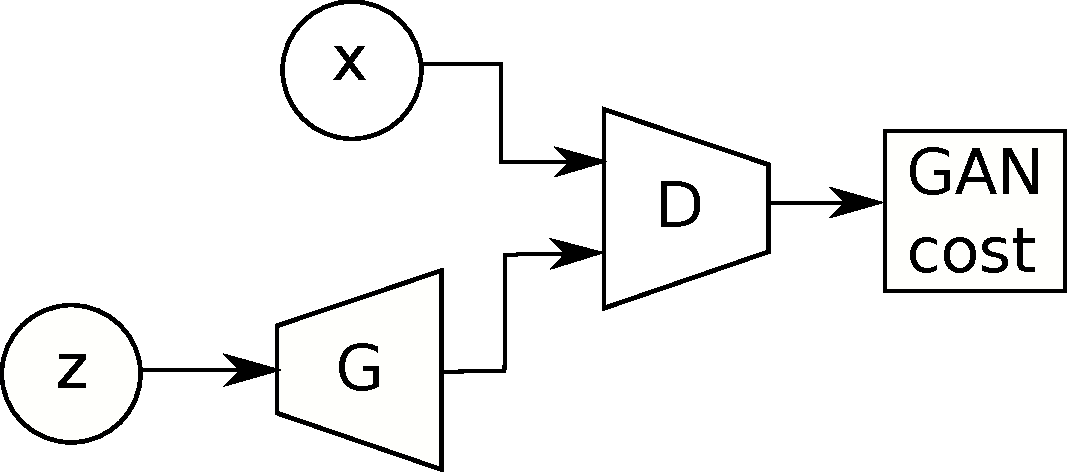
\includegraphics[width=\textwidth]{gan.pdf}
		\caption{GAN}
		\label{fig:gan}
	\end{subfigure}
	\begin{subfigure}[b]{0.45\textwidth}
		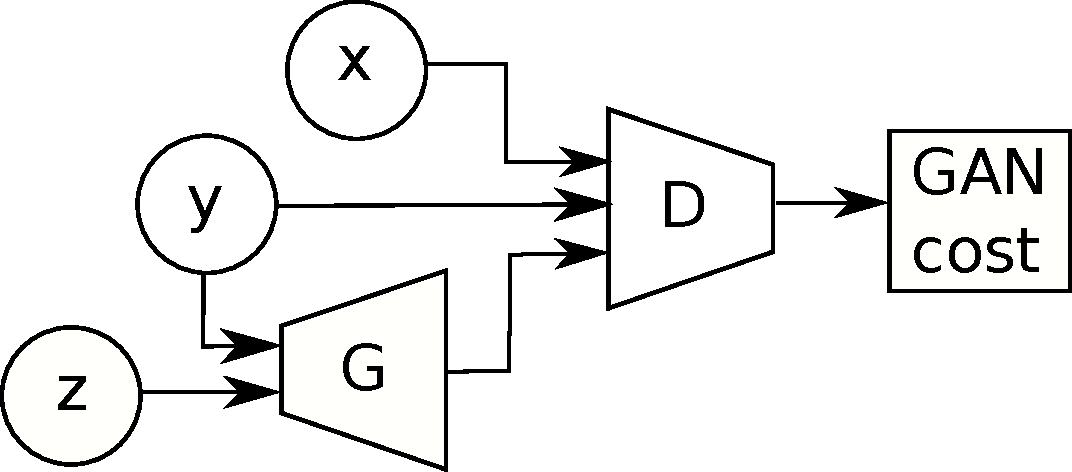
\includegraphics[width=\textwidth]{cgan.pdf}
		\caption{CGAN}
		\label{fig:cgan}
	\end{subfigure}
	\begin{subfigure}[b]{0.45\textwidth}
		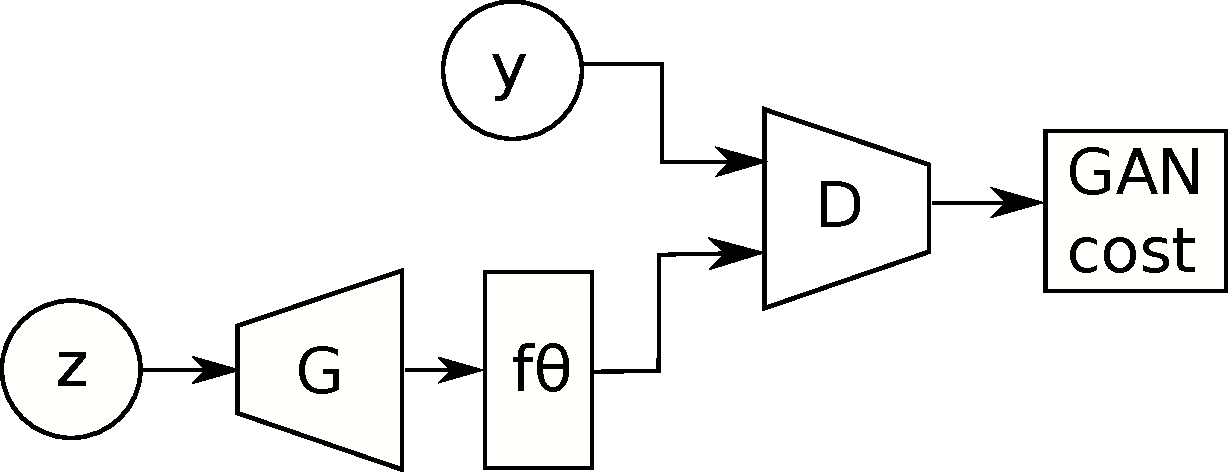
\includegraphics[width=\textwidth]{ambiantgan.pdf}
		\caption{AmbientGAN}
		\label{fig:ambientgan}
	\end{subfigure}
	\hspace{3mm}
	\begin{subfigure}[b]{0.45\textwidth}
		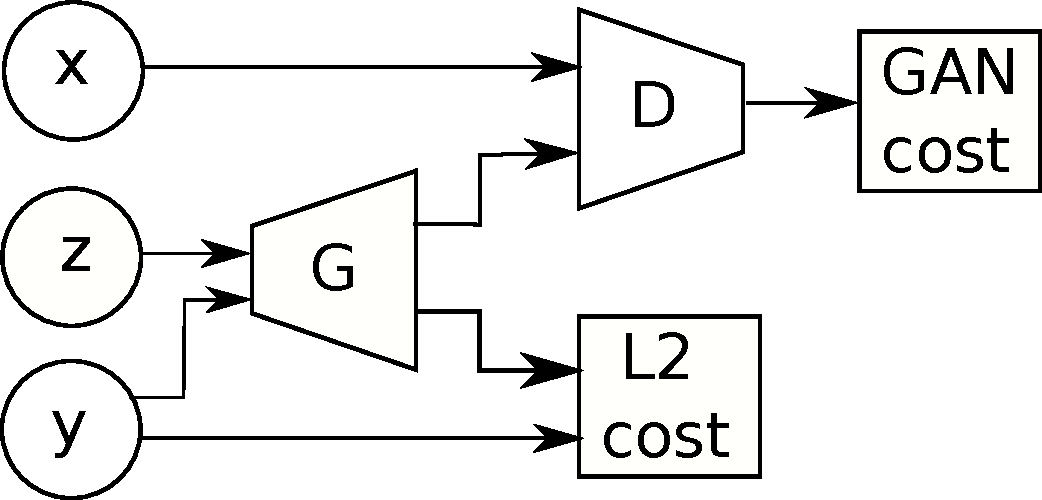
\includegraphics[width=\textwidth]{approach.pdf}
		\caption{Our approach}
		\label{fig:ourapproach}
	\end{subfigure}
	\caption[\ac{GANs} for image reconstruction]{Different GAN Setups. G and D are the generator and discriminator networks, x and z are samples from the distributions $\p{X}$ and $\p{r}$, y is a label/constraint map sampled from $\p{Y}$ and $f_\theta$ is an image degradation function.}
	\label{fig:gansetup}
\end{figure}

\subsection{Image reconstruction as a maximum a posteriori estimation}
\label{subs:maximum_a_posteriori}

We intend to learn a GAN whose generation network takes as input the constraint map $\vy$ and the sampled latent code $\vz \in \setZ$ and outputs a realistic image that fulfills the prescribed pixel values. Within this setup, the generative model can sample from the unknown distribution $\p{X}$ of the training images $\{x_1, \cdots, x_N\}$ while satisfying unseen pixel-wise constraints at training stage.  This approaches offers the advantages  of the two  aforementioned  families of methods, since it does not rely on per-sample optimization and provides a simple and efficient sampling mechanism through the latent variable $\vz$ while still providing a strong enforcing of the constraints. This allows for the efficient sampling of several potential solutions, which can be crucial in some applications \citep{Laloy2019}. 

Assuming that the constraint map is obtained through a noisy measurement process, we have
\begin{equation}
y = A\vx + \varepsilon \enspace.
\label{eq:noisy_generation_primary_CGAN}
\end{equation}
Here $A$ is the masking matrix yielding to $y = M(\vy) \odot \vx$, as seen in \citesec{sub:image_reconstruction_problem}. Also the constrained pixels are randomly and independently selected. $\varepsilon$ represents an additive i.i.d noise corrupting the pixels. Therefore we can formulate the Maximum A Posteriori (MAP) estimation problem, which, given the constraint map $y$, consists in finding the most probable image $x^*$ following the posterior distribution $\p{X|Y}$,
\begin{align}
x^* &= \arg\max_x\log {\p{X|Y}}\\
&= \arg\max_x\log \p{Y|X}+ \log \p{X} \enspace.
\label{eq:bayesian_formulation_our_primary_CGAN}
\end{align}

\noindent $p_{Y|X}(y|x)$ is the likelihood that the constrained pixels $y$ are issued from image $x$ while $\p{X}(x)$ represents the prior probability at $x$. Assuming that the generation network $G$ may sample the most probable image $G(y, z)$ complying with the given pixel values $y$, we get the following problem

\begin{equation}
G^* = \arg\max_G \mathop{\mathbb{E}}_{\substack{y\sim \p{Y}\\z\sim \p{Z}}} \log \p{Y|G(y, z)} + \log \p{G(y, z)} \enspace.
\label{eq:bayesian_formulation_our_primary_CGAN_G}
\end{equation}

\noindent The first term in Problem (\ref{eq:bayesian_formulation_our_primary_CGAN_G}) measures the likelihood of the constraints given a generated image. Let rewrite Equation (\ref{eq:noisy_generation_primary_CGAN}) as $\vect(y) = \vect(f_M(x)) + \vect(\varepsilon)$ where $\vect(\cdot)$ is the vectorisation operator that consists in stacking the constrained pixels. Therefore, assuming $\vect(\varepsilon)$ is i.i.d and follows a Gaussian distribution $\mathcal{N}(0,\sigma^2 I)$, we achieve the expression of the conditional likelihood
\begin{equation}
\log \p{y|G(y, z)} \, \propto - \left \|\vect(y) - \vect(M(y) \odot G(y,z))\right\|_2^2 \enspace
\end{equation}
\noindent which evaluates the quadratic distance between the conditioning pixels and their predictions by $G$. In other words, using a matrix notation of  (\ref{eq:noisy_generation_primary_CGAN}), the likelihood of the constraints given a generated image equivalently writes

\begin{equation}
\log {p_{Y|X}}(y|G(y, z) \, \propto - \left \|y - M(y) \odot G(y,z)\right\|_F^2 \enspace.
\end{equation}

\noindent $\| A \|_F^2 $ represents the squared Frobenius norm of matrix $A$ that is the sum of its squared entries. 
%
%In this work, we assume that $\epsilon$ follows a normal distribution $\epsilon\sim\mathcal{N}[0,\sigma^2]$, but it is worth noting that any prior distribution with a close-form solution for maximum likelihood estimation (typically distribution from the exponential family) can be used.
%In the case of the normal distribution, we can minimize our error term by using the $L_2$ norm on the constrained pixels.
%    

The second term in Problem (\ref{eq:bayesian_formulation_our_primary_CGAN_G}) is the likelihood of the generated image under the true but unknown data distribution $\p{X}$. Maximizing this term can be equivalently achieved by minimizing the distance between $\p{X}$ and the marginal distribution of the generated samples $G(y,z)$. This amounts to minimizing with respect to $G$, the GAN-like objective function $\mathop{\mathbb{E}}_{\substack{x\sim \p{X}}} \log(D(x)) + \mathop{\mathbb{E}}_{\substack{z\sim \p{Z}\\y\sim \p{Y}}} \log(1-D(G(y, z)))$  \citep{Goodfellow2014}. Putting altogether these elements, we can propose a relaxation of the hard constraint optimization problem (\ref{eq:formulation_our_primary_GAN}) (Figure \ref{fig:ourapproach}) as follows
%minimizing the Jensen-Shannon divergence between the real data distribution and the distribution of the generated data \citep{Goodfellow2014}.

%In our approach, we explicitly model the relaxation of the constraint by minimizing the $L_2$ norm between the constrained pixels and the generated values (see Fig.\ref{fig:ourapproach}).

%The objective function, with $\lambda \geq 0$ an additional parameter, becomes:
\begin{eqnarray}
\min_G \max_D L(D,G) & {\small=} & \mathop{\mathbb{E}}_{\substack{x\sim \p{X}}} \Big[\log(D(x))\Big] \label{eq:final_optim_problem} \\
&+&\mathop{\mathbb{E}}_{\substack{z\sim \p{Z}\\y\sim \p{Y}}} \Big[\log(1-D(G(y, z)))+\lambda \left\|y - M(y) \odot G(y,z)\right\|_F^2 \Big] \enspace . \nonumber
\end{eqnarray}

It is to note that the assumption of Gaussian noise measurement leads us to explicitly turn the pixel value constraints into the  minimization of the $\ell_2$ norm between the real enforced pixel values and their generated counterparts (see Figure \ref{fig:ourapproach}) as it corresponds to maximizing the likelihood of the pixels in the generated  image. The additional term acts as a regularization over prescribed pixels by the mask $M(y)$. The trade-off between the distribution matching loss and the constraint enforcement is assessed by the regularization parameter $\lambda \geq 0$. It is also worth noting that the noise $\varepsilon$ can be of any other distribution, according to the prior information, one may associate to the measurement process. We only require this distribution to admit a closed-form solution for the maximum likelihood estimation for optimization purpose. Typical choices are distributions from the exponential family \citep{Brown1986}.
	
\begin{figure}[t]
	\centering
	\begin{subfigure}[t]{0.25\textwidth}
		\centering
		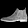
\includegraphics[scale=1.5]{origin.png}
		\caption{Original\\Image}
		\label{fig:original_shoe}
	\end{subfigure}\begin{subfigure}[t]{0.25\textwidth}
		\centering
		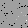
\includegraphics[scale=1.5]{consts.png}
		\caption{Constraints}
		\label{fig:constraints}
	\end{subfigure}\begin{subfigure}[t]{0.25\textwidth}
		\centering
		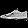
\includegraphics[scale=1.5]{img.png}
		\caption{Generated\\Image}
		\label{fig:pixelwise}
	\end{subfigure}\begin{subfigure}[t]{0.24\textwidth}
		\centering
		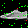
\includegraphics[scale=1.5]{imgcolor.png}
		\caption{Satisfied\\Consts.}
		\label{fig:generated}
	\end{subfigure}
	\caption[Generation of a sample during training]{Generation of a sample during training. We first sample an image from a training set (\ref{fig:original_shoe}) and we sample the constraints (\ref{fig:constraints}) from it. Then our GAN generates a sample (\ref{fig:pixelwise}). The constraints with squared error smaller than $\epsilon=0.1$ are deemed satisfied and shown by green pixels in (\ref{fig:generated}) while the red pixels are unsatisfied.}
	\label{fig:image_completion}
\end{figure}

\subsection{Conditioning with an auxiliary task}

To solve Problem (\ref{eq:final_optim_problem}), we use the stochastic gradient descent method. The overall training procedure is detailed in Algorithm \ref{alg:train} and ends up when a maximal number of training epochs is attained. 

\begin{algorithm}[!ht]
	\caption{Proposed training algorithm}
	\label{alg:train}
	\begin{algorithmic}[H]
		\REQUIRE{ $\trainsetX$ the set of  unaltered images, $\trainsetY$ the set of constraint maps, $G$ the generation network, and $D$ the discrimination function}
		\REPEAT
		\STATE sample a mini-batch $\lbrace x_i \rbrace_{i=1}^m$ from $\trainsetX$\;
		\STATE sample a mini-batch $\lbrace y_i \rbrace_{i=1}^m$ from $\trainsetY$\;
		\STATE sample a mini-batch $\lbrace z_i \rbrace_{i=1}^m$ from distribution $\p{Z}$ \;
		\STATE update $D$ by stochastic gradient ascent of
		\STATE \ \ \ \ $ \sum_{i=1}^{m}\log(D(x_i)) + \log(1-D(G(y_i, z_i)))$
		\STATE sample a mini-batch $\lbrace y_j \rbrace_{j=1}^n$ from $\trainsetY$\;
		\STATE sample a a mini-batch $\lbrace z_j \rbrace_{j=1}^n$ from distribution $\p{Z}$\;; 
		\STATE update $G$ by stochastic gradient descent of
		\STATE \ \ \ \ $ \sum_{j=1}^n \log(1-D(G(y_j, z_j))) + ||y_j - M(y_j)\odot G(y_j, z_j)||_F^2$\;
		\UNTIL a stopping condition is met
		
	\end{algorithmic}
\end{algorithm}

When implementing this training procedure we experienced, at inference stage, a lack of diversity in the generated samples (see Figure \ref{fig:diversity_loss}) with deeper architectures, most notably the encoder-decoder architectures. This issue manifests itself through the fact that the learned generation network, given a constraint map $y$, outputs almost deterministic image  regardless the variations in the input $z$. The issue was also pointed out by Yang et al. \citep{Yang2019} as characteristic of CGANs.

To avoid the problem, we exploit the PacGAN \citep{Lin2018} technique: it consists in passing a set of samples to the discrimination function instead of a single one.  PacGAN is intended to tackle the mode collapse problem in GAN training. The underlying principle being that if a set of images are sampled from the same training set, they are very likely to be completely different, whereas if the generator experiences mode collapse, generated images are likely to be similar.
In practice, we only give two samples to the discriminator, which is sufficient to overcome the loss of diversity as  suggested in \citep{Lin2018}. 
%
The resulting training procedure is summarized in Algorithm~\ref{alg:trainpac}.

\begin{algorithm}[!ht]
	\caption{Our training algorithm including PacGAN}
	\label{alg:trainpac}
	\begin{algorithmic}[H]
		\REQUIRE { $\trainsetX$ the set of  unaltered images, $\trainsetY$ the set of constraint maps, $G$ the generation network, and $D$ the discrimination function}
		\REPEAT
		\STATE sample two mini-batches $\lbrace x_i^a \rbrace_{i=1}^m$, $\lbrace x_i^b\rbrace_{i=1}^m$ from $\trainsetX$\;
		\STATE sample a mini-batch $\lbrace y_i \rbrace_{i=1}^m$ from $\trainsetY$\;
		\STATE sample two mini-batches $\lbrace z_i^a \rbrace_{i=1}^m$, $\lbrace z_i^b \rbrace_{i=1}^m$ from distribution $\p{Z}$ \;
		\STATE update $D$ by stochastic gradient ascent of
		\STATE \ \ \ \ $ \sum_{i=1}^{m}\log(D(x_i^a, x_i^b)) + \log(1-D(G(y_i, z_i^a), G(y_i, z_i^b)))$
		\STATE sample a mini-batch $\lbrace y_j \rbrace_{j=1}^n$ from $\trainsetY$\;
		\STATE sample two mini-batches $\lbrace z_i^a \rbrace_{i=1}^m$, $\lbrace z_i^b \rbrace_{i=1}^m$ from distribution $\p{Z}$ \;
		\STATE update $G$ by stochastic gradient descent of
		\STATE \ \ \ \ $ \sum_{j=1}^n \log(1-D(G(y_j, z_j))) + ||y_j - M(y_j)\odot G(y_j, z_j)||_F^2$\;
		\UNTIL a stopping condition is met
		
	\end{algorithmic}
\end{algorithm}


\FloatBarrier

\section{Experimental results and application}

\subsection{Experimental setting} \label{sec:experiments_protocol}
We have conducted a series of empirical evaluation to assess the performances of the proposed GAN. Used datasets, evaluation protocol and the tested deep architectures are detailed in this section while Section \ref{sec:results} is devoted to the results presentation. 
\subsubsection{Datasets}

We tested our approach on several datasets listed hereafter. Detailed  information on these datasets are provided  in the Appendix \ref{app:det_datasets}.
%namely FashionMNIST \citep{Xiao2017}, CIFAR10 \citep{Krizhevsky2009CIFAR10}, CelebA\citep{liu2015celeba} and a custom-made Texture texture dataset:
\begin{description}
	\item{FashionMNIST} \citep{Xiao2017} consists of 60,000 $28\times 28$ small grayscale images of fashion items, split in 10 classes and is a harder version of the classical MNIST  dataset \citep{LeCun1998a}. %known to be simple to solve. 
	The very small size of the images makes them particularly appropriate for large-scale experiments, such as hyper-parameter tuning. 
	
	\item{CIFAR10} \citep{Krizhevsky2009} consists of 60,000 $32 \times 32$ colour images of 10 different and varied classes. It is deemed less easy than MNIST and FashionMnist.
	%considered harder to learn that MNIST and FashionMNIST, even it is of nearly the same dimension.
	\item{CelebA}\citep{Liu2015} is a large dataset of celebrity portraits labeled by identity and a variety of binary features such as eyeglasses, smiling... We use 100,000 images cropped to a size of $128 \times 128$, making this dataset appropriate for a high dimension evaluation of our approach in comparison with related work.
	
	\item{Texture} is a custom dataset 
	%was eventually created that is composed of texture, sampling $20000$ patches
	composed of $20,000$ $160 \times 160$ patches sampled from a large brick wall texture, as recommended in \citep{Jetchev2017}. It is worth noting that this procedure can be reproduced on any texture image of sufficient size. Texture is a testbed of our approach on fully-convolutional networks for constrained texture generation task. 
	%This allows us to experiment fully-convolutional architectures on a texture reconstruction task.
	
	\item{Subsurface} is a classical dataset in geological simulation \citep{Strebelle2002} which consists, similarly to the Texture dataset, of 20,000  $160 \times 160$ patches sampled from a model of a subsurface binary domain. These models are assumed to have the same properties as a texture, mainly the property of global ergodicity of the data.
	
	
\end{description}

To avoid learning explicit pairing of real images seen by the discrimination function with constraint maps provided to the generative network, we split each dataset into training, validation and test sets, to which we add a set composed of constraint maps that should remain unrelated to the three others.
In order to do so, a fifth of each set is used to generate the constrained pixel map $y$ by randomly selecting $0.5\%$ of the pixels from a uniform distribution, composing a set of constraints for each of the train, test and validation sets. The images from which these maps are sampled are then removed from the training, testing and validation sets. For each carried experiment the best model is selected based on some performance measures (see Section \ref{subs:eval}) computed on the validation set. Finally, reported results are computed on the test set.

%To avoid learning explicit correlations between real examples presented to the discriminator and constraint maps given to the generator, we create a splitting consisting in the classical train, validation and test databases, to which we add a constraints database that should remain unrelated to the three others. A fifth of each set is used to generated the matrix of constraints $C$ by randomly selecting $0.5\%$ of the pixels, uniformly. These images are then removed from the training, testing and validation sets.


\subsubsection{Network architectures}
\label{subs:architectures}

We use a variety of GAN architectures in order to adapt to the different scales and image sizes of our datasets. The detailed configuration of these architectures are exposed in Appendix \ref{app:det_archis}.

For the experiments on the FashionMNIST \citep{Xiao2017}, we use a lightweight network for both the discriminator and the generator similarly to DCGAN  \citep{Radford2015} due to the small resolution of FashionMnist images.
%This is motivated by the large number of experiments and the small dimension of the images.

To experiment on the Texture dataset, we consider a set of fully-convolutional generator architectures based on either dilated convolutions \citep{Yu2015}, which behave well on texture datasets \citep{Ruffino2017}, or encoder-decoder architectures that are commonly used in domain-transfer applications such as CycleGAN \citep{Zhu2017}. We selected these architectures because they have very large receptive fields without using pooling, which allow the generator to use a large context for each pixel.

We keep the same discriminator across all the experiments with these architectures, the PatchGAN discriminator \citep{Isola2016}, which is a five-layer fully-convolutional network with a sigmoid activation.

The Up-Dil architecture consists in a set of transposed convolutions (the upscaling part), and a set of dilated convolutional layers \citep{Yu2015}, while the Up-EncDec has an upscaling part followed by an encoder-decoder section with skip-connections, where the constraints are downscaled, concatenated to the noise, and re-upscaled to the output size.

The UNet \citep{Ronneberger2015} architecture is an encoder-decoder where skip-connections are added between the encoder and the decoder.
The Res architecture is an encoder-decoder where residual blocks \citep{He2015} are added after the noise is concatenated to the features. The UNet-Res combines the UNet and the Res architectures by including both residual blocks and skip-connections.

Finally, we will evaluate our approach on the Subsurface dataset using the architecture that yields to the best performances on the Texture dataset.
%
\subsubsection{Evaluation}

\label{subs:eval}
We evaluate our approach based on both the satisfaction of the pixel constraints and the visual quality of sampled images. From the assumption of Gaussian measurement noise (as discussed in Section \ref{sec:our-approach}), we assess the constraint fulfillment using the following mean square error (MSE) 
\begin{equation}
MSE = \frac{1}{L} \sum_{i=1}^L \left\|y_i - M(y_i) \odot G(y_i, z_i)\right\|_F^2
\end{equation}
This metric should be understood as the mean squared error of reconstructing the constrained pixel values. 

Visual quality evaluation of an image is not a trivial task \citep{Theis2015}. However, Fréchet Inception Distance (FID) \citep{Heusel2017} and Inception Score \citep{Salimans2016}, have been used to evaluate the performance of generative models. We employ FID since the Inception Score has been shown to be less reliable \citep{Barratt2018}. Since the FID requires a pre-trained classifier adapted to the dataset in study, we trained simple convolutional neural networks as classifiers for the FashionMNIST and the CIFAR-10 datasets. For the Texture dataset, since the dataset is not labeled, we resort to a CNN classifier trained on the Describable Textures Dataset (DTD) \citep{Cimpoi2014}, which is a related application domain.

However, since we do not have labels for the Subsurface dataset, we could not train a classifier for this dataset, thus we cannot compute the FID. To evaluate the quality of the generated samples, we use metrics based on a distance between feature descriptors extracted from real samples and generated ones. Similarly to \citep{Ruffino2017}, we rely on a $\chi^2$ distance between the Histograms of Oriented Gradients (HOG) or Local Binary Patterns (LBP) features computed on generated and real images. 

Histograms of Oriented Gradients (HOG) \citep{Dalal2005} and Local Binary Patterns (LBP) \citep{Pietikainen2011} are computed by splitting an image into cells of a given radius and computing on each cell the histograms of the oriented gradients for HOGs and of the light level differences for each pixel to the center of the cell for LBPs.  Additionally, we consider the domain-specific metric, the connectivity function \citep{Lemmens2017} which is presented in Appendix \ref{app:geostatistics}.

Finally, we check by visual inspection if the trained model $G$ is able to generate diverse samples, meaning that for a given $y$ and for a set of latent codes $(z_1, ..., z_n) \sim \p{Z}$, the generated samples $G(y,z_1), \ldots, G(y, z_n)$ are visually different. 

%Since we empirically observed that our models were either producing very different samples or samples that only differ by a small noise factor, we do not propose a specific evaluation metric and instead check manually if a loss of diversity occurs.


\subsection{Quality-fidelity trade-off}
\label{subs:results}

% \begin{figure}[!]
%     \centering
%     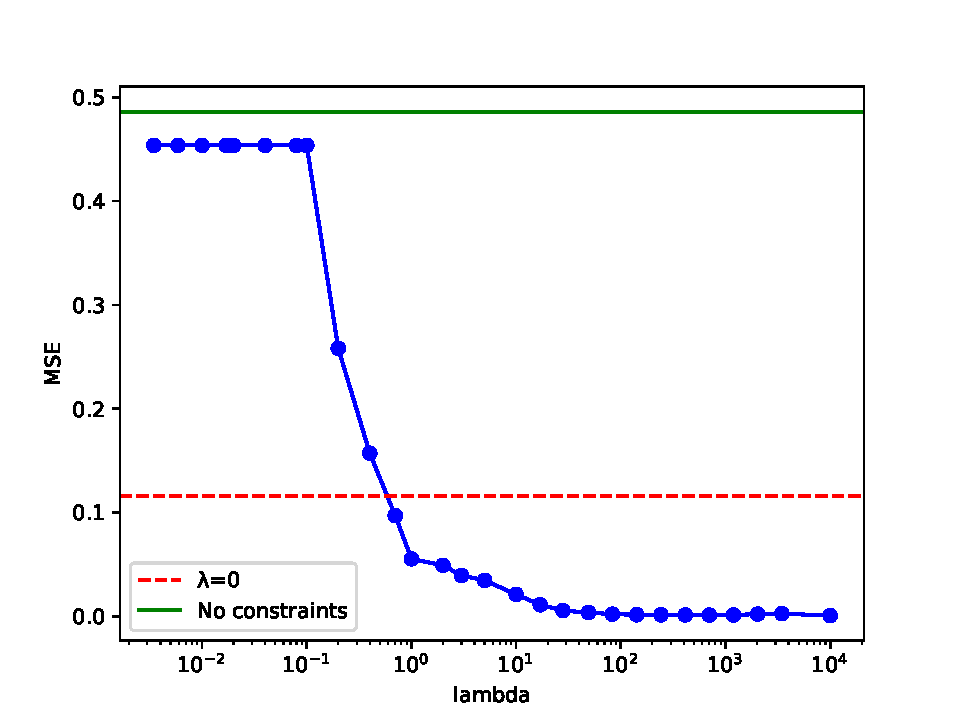
\includegraphics[trim=0 0 0 40, clip,scale=0.35]{MSE_mnist}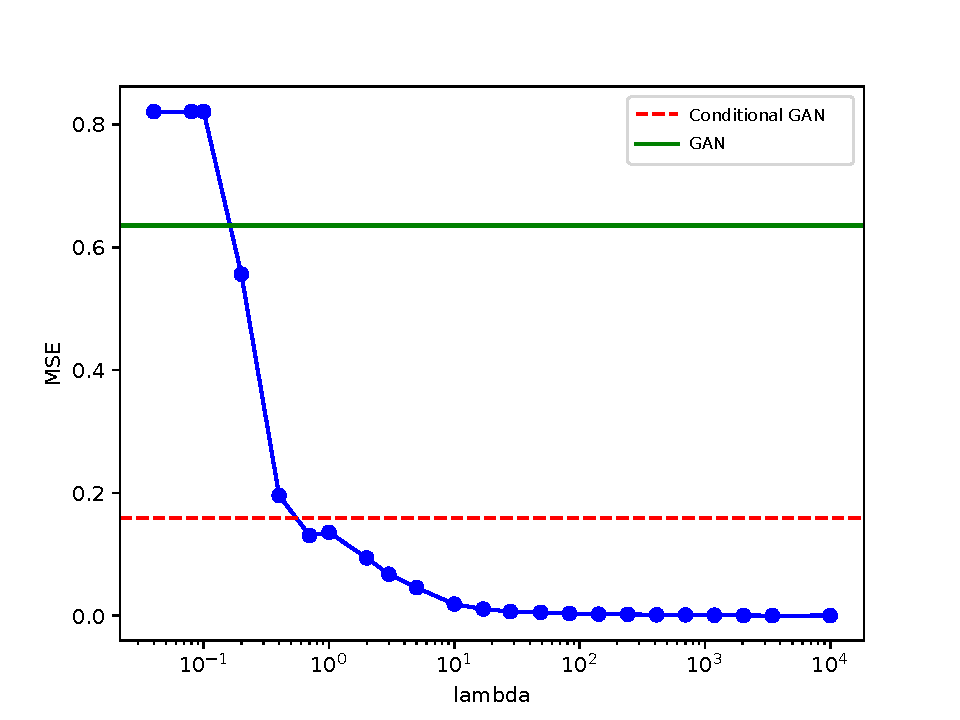
\includegraphics[trim=0 0 0 40, clip,scale=0.35]{MSE_fashion}
%     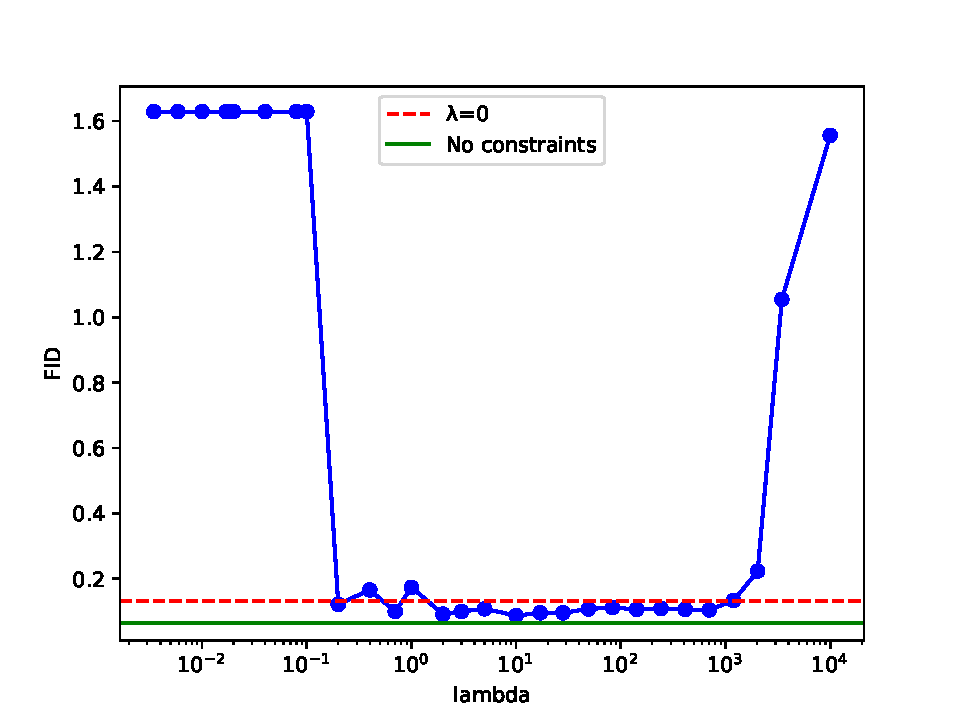
\includegraphics[trim=0 0 0 40, clip,scale=0.35]{FID_mnist}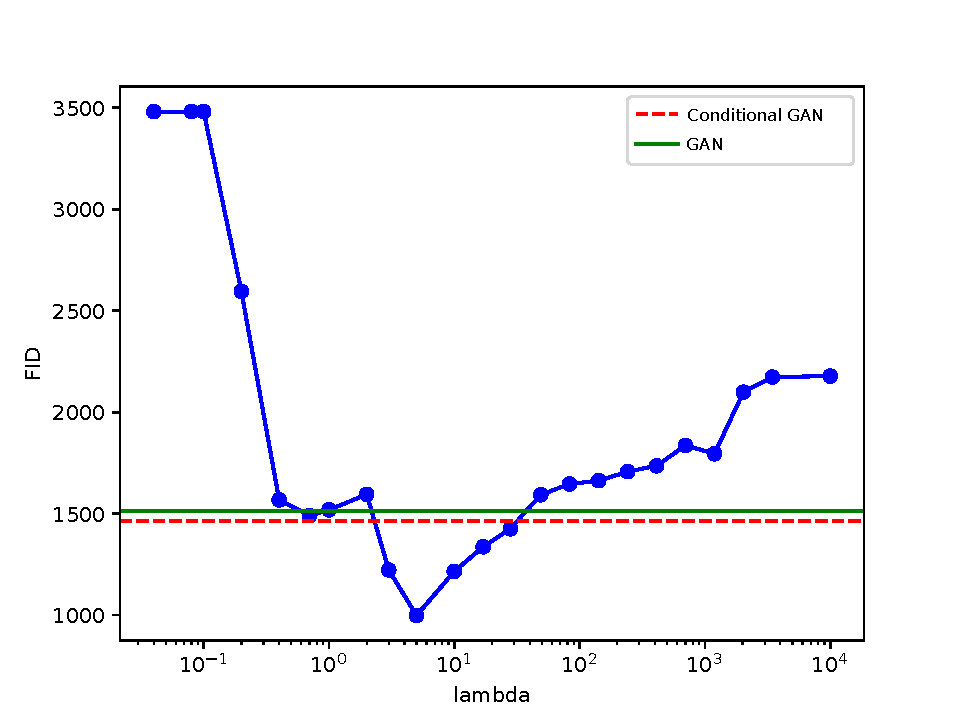
\includegraphics[trim=0 0 0 40, clip,scale=0.35]{FID_fashion}

%     \centering
%     \caption{MSE (top) and  FID (bottom) w.r.t. the regularization parameter $\lambda$;
%     Dataset MNIST (left), Fashion MNIST (right).
%     %The different orders of magnitude for the Y-axis of the FID is due to the different classifiers used to compute this distances.
%     }
%     \label{fig:fids}
%     \label{fig:mses}
% \end{figure}

\begin{figure}[t]
	\centering
	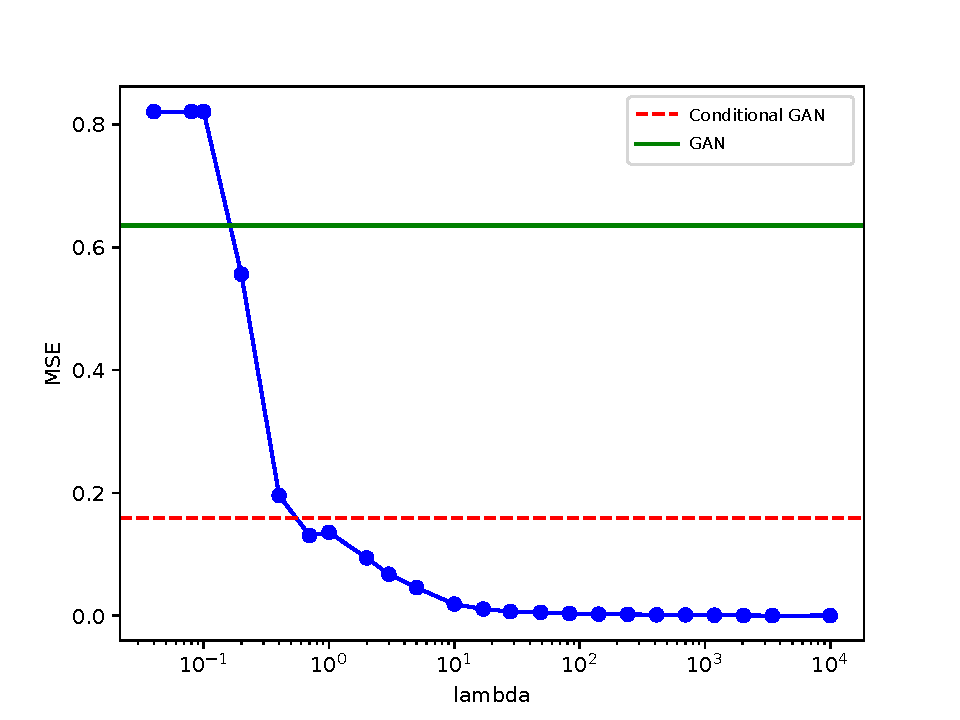
\includegraphics[trim=0 0 0 40, clip,scale=0.4]{MSE_fashion}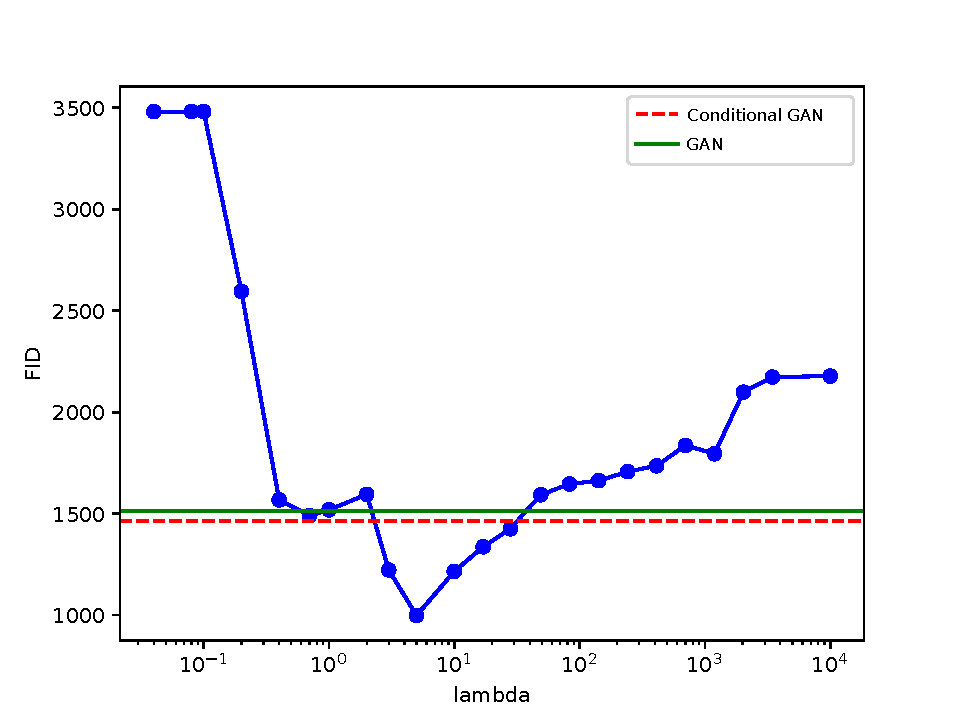
\includegraphics[trim=0 0 0 40, clip,scale=0.4]{FID_fashion}
	
	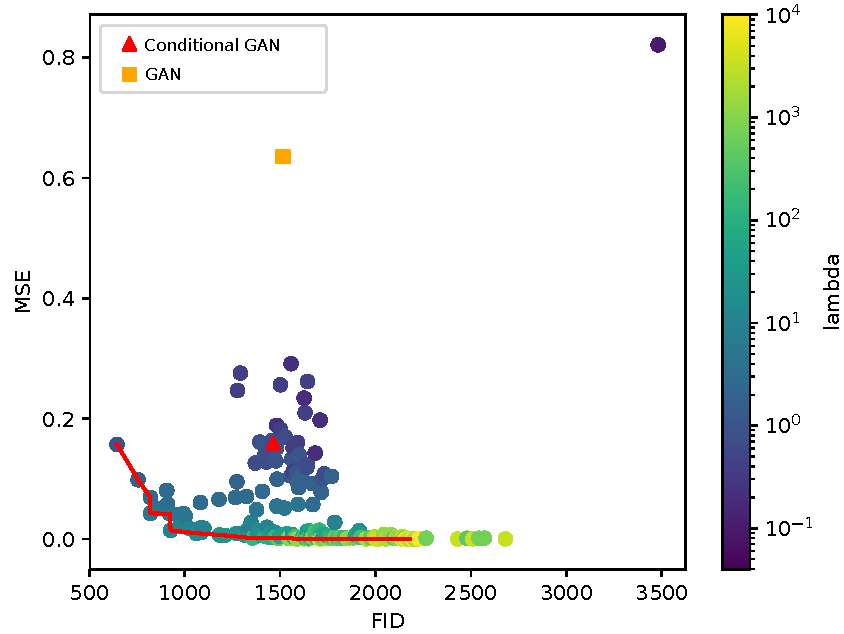
\includegraphics[scale=0.5]{pareto_fashion}
	
	\centering
	\caption[Comparison between our approach and the GAN/CGAN approach on FashionMNIST]{Our approach compared to the GAN and CGAN baselines. MSE (left) and  FID (right) w.r.t. the regularization parameter $\lambda$, MSE w.r.t the FID (bottom).
		%The different orders of magnitude for the Y-axis of the FID is due to the different classifiers used to compute this distances.
	}
	\label{fig:fids}
	\label{fig:mses}
	\label{fig:paretos}
\end{figure}

%In this set of experiments, 
We first study the influence of the $\lambda$ regularization hyper-parameter on both the quality of the generated samples and the respect of the constraints. We experiment on the %MNIST \citep{Lecun1998} and
FashionMNIST \citep{Xiao2017} dataset, since such a study requires intensive simulations permitted by the low resolution of FashionMnist images and the used architectures (see Section \ref{subs:architectures}). 
%a lot of re-training and the small size of the images allowed us to run several hundreds of experiments.

To overcome classical GANs instability, the networks are trained 10 times and the median values of the best scores on the test set at the best epoch 
are recorded. The epoch that minimizes:
\begin{equation*}
\sqrt{\left(\frac{FID - FID_{min}}{FID_{max}- FID_{min}}\right)^2 + \left(\frac{MSE - MSE_{min}}{MSE_{max}- MSE_{min}}\right)^2}
\end{equation*}  on the validation set is considered as the best epoch, where $FID_{min}$, $MSE_{min}$, $FID_{max}$ and $MSE_{max}$ are respectively the lowest and highest FIDs and MSEs obtained on the validation set.

Empirical evidences (highlighted in Figure \ref{fig:mses}) show that with a good choice of $\lambda$, the regularization term helps the generator to enforce the constraints, leading to smaller MSEs than when using the CGAN ($\lambda=0$) without compromising on the quality of generated images. Also, we can note that using the regularization term even leads to a better image quality compared to GAN and CGAN.
%
The bottom panel in Figure \ref{fig:paretos} illustrates that the trade-off between image quality and the satisfaction of the constraints can be controlled by appropriately setting the value of $\lambda$. Nevertheless, for small values of $\lambda$ (less or equal to $10^{-1}$), our GAN model fails to learn meaningful distribution of the training images and only generates uniformly black images. This leads to the plateaus on the MSE and FID plots (top panels in Figure \ref{fig:mses}).


% \begin{figure}
%     \centering
%     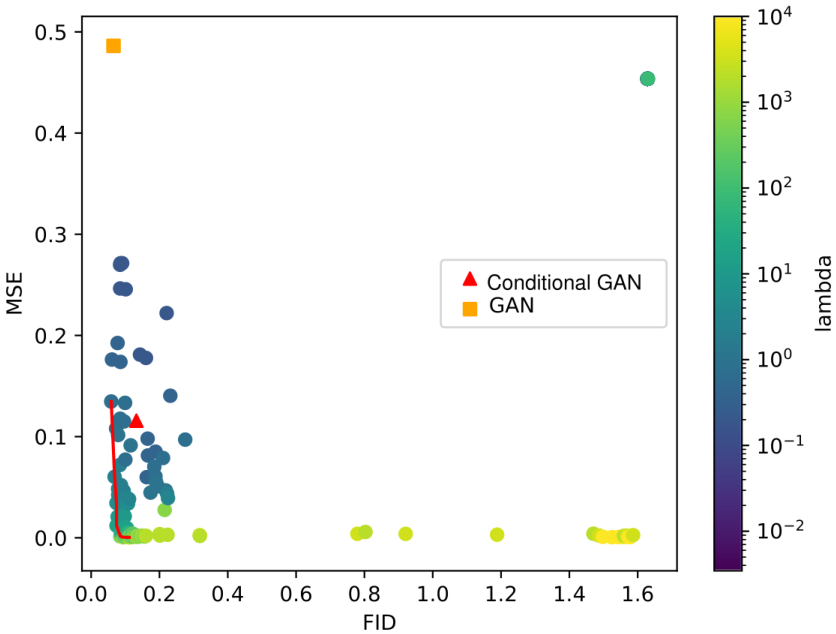
\includegraphics[trim=0 0 0 40, clip,scale=0.4]{pareto_mnist}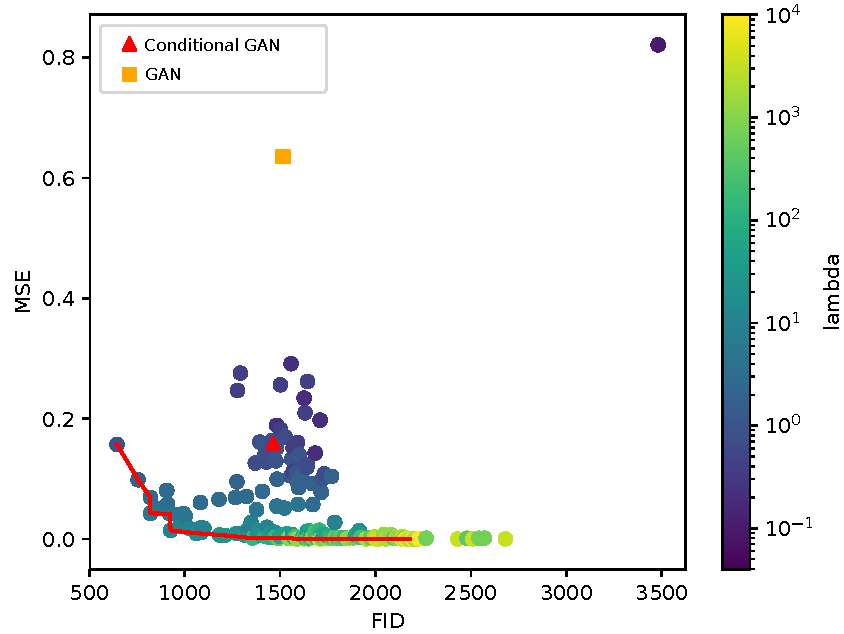
\includegraphics[trim=0 0 0 40, clip,scale=0.4]{pareto_fashion}
%     \vspace*{-3mm}
%     \caption{MSE w.r.t the FID. Left: MNIST; Right: Fashion MNIST. Note that due to the failure mode previously mentioned, a large part of the values are stacked in the top right corner of these figures.
%     }
%     \label{fig:paretos}
% \end{figure}  

\subsection{Texture generation with fully-convolutional architectures}
\label{sub:fcnn}
Fully-convolutional architectures for GANs are widely used, either for domain-transfer applications \citep{Zhu2017}\citep{Isola2016} or for texture generation \citep{Jetchev2017}. In order to evaluate the efficiency of our method on relatively high resolution images, we experiment the fully-convolutional networks described in Section \ref{subs:architectures} on a texture generation task using Texture dataset. We investigate the upscaling-dilatation network, the encoder-decoder one and the resnet-like architectures.

Our training algorithm was run for 40 epochs on all reported results. We provide a comparison to CGAN\citep{Mirza2014} approach by using the selected best architectures.
The models are evaluated in terms of best FID (visual quality of sampled images) at each epoch and MSE (conditioning on fixed pixel values).  We also compute the FID score of the models at the epochs where the MSE is the lowest. In the other way around, the MSE is reported at epoch when the FID is the lowest. The obtained quantitative results are detailed in Table \ref{tab:ablation}.

For the encoder-decoder models, we can notice that the models using ResNet blocks perform better than just using a UNet generator. A trade-off can also be seen between the FID and MSE for the ResNet models and the UNet-ResNet, which could mean that skip-connections help the generator to fulfill the constraints but at the price of lowered visual quality.

Although the encoder-decoder models perform the best, they tend to lose diversity in the generated samples (see Figure \ref{fig:diversity_loss}), whereas the upscaling-based models have high FID and MSE but naturally preserve diversity in the generated samples.

\begin{figure}
	\centering
	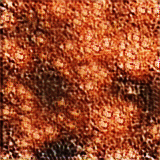
\includegraphics[width=2cm]{diversity_1.png}\hspace{0.5cm}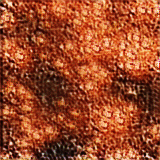
\includegraphics[width=2cm]{diversity_2.png}\hspace{0.5cm}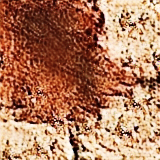
\includegraphics[width=2cm]{diversity_1_pac.png}\hspace{0.5cm}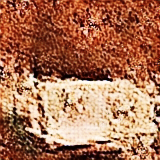
\includegraphics[width=2cm]{diversity_2_pac.png}
	
	\vspace{0.3cm}
	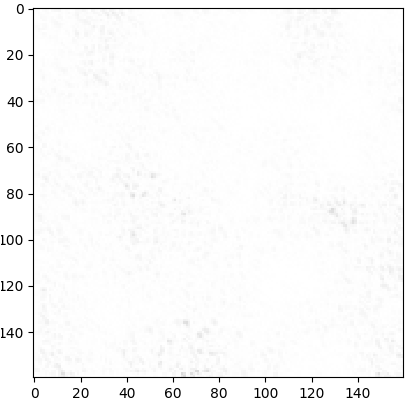
\includegraphics[height=4cm]{diversity_diff_nobar.png}\hspace{0.5cm}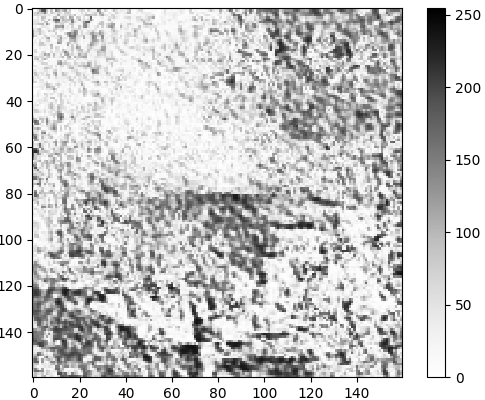
\includegraphics[height=4cm]{diversity_diff_pac.png}
	\caption[An example of a loss of diversity]{An example of a loss of diversity when generating Texture samples with a trained UNetRes network using two different random noises $z$ and a single constraint map $y$. The two samples on the top left are generated using the classical GAN discriminator whereas the samples on the top right are generated using the PacGAN approach. The loss of diversity is clearly visible on the absolute differences between the greyscaled images (bottom).}
	\label{fig:diversity_loss}
\end{figure}

Changing the discriminator for a PacGAN discriminator with 2 samples in the encoder-decoder based architectures allows to restore diversity, while keeping the same performances as previously or even increasing the performances for the UNetRes (see Table \ref{tab:ablation}).

Table \ref{tab:ablation-cgan} compares our proposed approach to CGAN using fully convolutional networks. It shows that our approach is more able to comply with the pixel constraints while producing realistic images. Indeed, our approach outperforms CGAN (see Table \ref{tab:ablation-cgan}) by a large margin on the respect of conditioning pixels (see the achieved MSE metrics by  our UNetPAC or UNetResPAC)  and gets  close FID performance on the generated samples. This finding is in accordance of the obtained results on FashionMnist experiments.
%show that the comparison with the CGAN approach still holds well in a fully-convolutional setting since our approach outperforms CGAN by a large margin on the respect of the constraints and come close to it on the visual quality of the generated samples. This conforms the results obtained on the previous experiments on the FashionMNIST dataset.

\begin{table}
	\centering
	\begin{tabular}{|l|c|c|c|c|c|}
		\hline
		Model           & Best FID & Best MSE & FID at & MSE at & Diversity\\
		&&&best MSE & best FID & \\
		\hline
		Up-Dil      & 0.0949 & 0.4137 & 1.0360 & 0.7057 & {\color{green}\cmark } \\
		Up-EncDec  & 0.1509 & 0.7570 & 0.2498 & 0.9809 & {\color{green}\cmark } \\
		UNet        & 0.0442 & 0.1789 & 0.0964 & 0.4559 & {\color{red}\xmark } \\
		Res      & 0.0458 & 0.0474 & 0.0590 & 0.0476 & {\color{red}\xmark } \\
		UNetRes & 0.0382 & 0.0307 & 0.0499 & 0.0338 & {\color{red}\xmark } \\
		\hline
		ResPAC &  \textbf{0.0350} & 0.0698 & 0.0466 & 0.4896 & {\color{green}\cmark } \\
		UNetPAC &  0.0672 & \textbf{$\leq$ 0.0001} & 0.3120 & 0.2171&  {\color{green}\cmark } \\
		UNetResPAC & 0.0431 & 0.0277 & \textbf{0.0447} & \textbf{0.0302} &  {\color{green}\cmark }\\
		\hline
	\end{tabular}
	
	\caption[Results on the Texture dataset for all the selected architectures]{Results obtained by the different fully-convolutional architectures on the Texture dataset. We can remark that the encoder-decoder greatly outperforms the upscaling ones and that using the PacGAN technique helps keeping the performance of these models while restoring the diversity in the samples. The bottom part of the table refers to PacGan architectures.}
	\label{tab:ablation}
\end{table}

\begin{table}[t]
	\centering
	\begin{tabular}{|l|c|c|c|c|c|}
		\hline
		Model           & Best FID & Best MSE & FID at & MSE at \\
		&&&best MSE & best FID  \\
		\hline
		CGAN-ResPAC &   \textbf{0.0234} & 0.1337 &  \textbf{0.0340} & 0.2951 \\
		CGAN-UNetPAC &  0.0518 & 0.2010 & 0.0705 & 0.4828\\
		CGAN-UNetResPAC & 0.0428 & 0.1060 & 0.0586 & 0.2250\\
		\hline
		Ours-ResPAC &  0.0350 & 0.0698 & 0.0466 & 0.4896\\
		Ours-UNetPAC &  0.0672 & \textbf{$\leq$ 0.0001}  & 0.3120 & 0.2171 \\
		Ours-UNetResPAC & 0.0431 & 0.0277 &0.0447 & \textbf{0.0302}\\
		\hline
	\end{tabular}
	
	\caption{Results obtained by the selected best fully-convolutional architectures on the Texture dataset for both the CGAN approach and our approach.}
	\label{tab:ablation-cgan}
\end{table}

\subsection{Extended architectures}
We extend the comparison of our approach to CGAN on the CIFAR10 and CelebA  datasets (Table \ref{tab:cifar10}). We investigated the architectures described in Section \ref{subs:architectures}. All reported results are obtained with the regularization parameter fixed to $\lambda=1$.
We train the networks for 150 epochs using the same dataset split as stated previously in order to keep independence between the images constraint maps. The evaluation procedure remains also unchanged. We use the PacGAN approach to avoid the loss of diversity issues. The experiments on both datasets show that though CGAN  provides better results in terms of visual quality, our approach outperforms it according to the respect of the pixel constraints.

\begin{table}[!]
	\centering
	\begin{tabular}{|l|c|c|c|c|c|}
		\hline
		&Model           & Best FID & Best MSE & FID at & MSE at \\
		&&&&best MSE & best FID \\
		\hline
		CIFAR-10 &CGAN   & \textbf{2,68}  & 0.081  & \textbf{2.68}  & 0.081\\
		&Ours            & 3.120 & \textbf{0.010} & 3.530 & \textbf{0.011} \\    
		\hline
		CelebA &CGAN      & \textbf{1.34e-4} & 0.0209 &  \textbf{1.81e-4} & 0.0450\\
		&Ours            & 2.09e-4& \textbf{0.0053} & 5.392e-4 & \textbf{0.0249} \\
		\hline
	\end{tabular}
	
	\caption{Results on the CIFAR10 and CelebA datasets. The reported performances compare CGAN to our proposed GAN conditioned on scarce constraint map.}
	\label{tab:cifar10}
\end{table}


\vspace{0.4cm}

\subsection{Application to hydro-geology}
\label{subs:subsurface}

\begin{table}
	\centering
	\begin{tabular}{|l|c|c|c|c|c|}
		\hline
		&Model           & Best HOG & Best MSE& HOG at & MSE at \\
		&&& &  best MSE & best HOG \\
		\hline
		Subsurface &CGAN   & \textbf{2.92e-4} & 0.2505 & \textbf{3.06e-4}  & 1.1550 \\
		&Ours            & 4.31e-4 & \textbf{0.0325}& 5.69e-4 & \textbf{0.2853} \\
		\hline
	\end{tabular}
	\caption{Evaluation of the trade-off between the visual quality of the generated samples and the respect of the constraints for the CGAN approach and ours on the Subsurface dataset.}
	\label{tab:subsurface}
\end{table}

\begin{table}[h]
	\centering
	\begin{tabular}{|l|c|c|c|c|c|}
		\hline
		&Model           & Best HOG & Best MSE& Best LBP & Best LBP \\
		&&& & (radius=1) & (radius=2) \\
		\hline
		Subsurface &CGAN   & \textbf{2.92e-4} & 0.2505 & \textbf{2.157} & \textbf{3.494}\\
		&Ours            &  4.31e-4 &\textbf{0.0325} & 10.142 & 16.754 \\
		\hline
	\end{tabular}
	\caption{Evaluation of the visual quality between the CGAN approach and ours on the Subsurface dataset using several metrics.}
	\label{tab:subsurface_visual}
\end{table}

Finally, we evaluate our approach on the Subsurface dataset. We use the UNetResPAC  architecture, since it performed the best on Texture data as exposed in Section \ref{sub:fcnn}. As previously, we simply set the regularization parameter at $\lambda=1$ and, the network is trained for 40 epochs using the same experimental protocol. To evaluate the trade-off between the visual quality and the respect of the constraints, instead of FID we rather compute distances between visual Histograms of Oriented Gradients (see Section \ref{sec:experiments_protocol}), extracted from real and generated samples. We also evaluate the visual quality of our approach with a distance between Local Binary Patterns. Indeed, Subsurface application lacks labelled data in order to learn a deep network classifier from which the FID score can be computed. 

%As stated before in Section \ref{subs:eval}, we cannot use the FID to evaluate the visual quality of the generated images since we don't have a supervised task linked to the data.
%Therefore we use distances between visual features, namely Histograms of Oriented Gradients and Local Binary Patterns (see Section \ref{sec:experiments_protocol}), extracted from real and generated samples.

The obtained results are summarized in Tables \ref{tab:subsurface} and \ref{tab:subsurface_visual}. They are coherent with the previous experiments since the generated samples are diverse and have a low error regarding the constrained pixels. The conditioning have a limited impact on the visual quality of the generated samples and compares well to unconditional approaches \citep{Ruffino2017}. Evaluation of the generated images using the domain-connectivity function highlights this fact on Figure \ref{fig:ours_connectivity} in the supplementary materials. Also examples of generated images by our approach  pictured in Figure \ref{fig:samples_subsurface} (see appendix \ref{app:generated_images}) show that we preserve the visual quality and honor the constraints.


\section{Conclusion and discussion}

In this chapter, we address the task of learning effective generative adversarial networks when only very few pixel values are known beforehand. To solve this pixel-wise conditioned GAN, we model the conditioning information under a probabilistic framework. This leads to the maximization of the likelihood of the constraints given a
generated image. Under the assumption of a Gaussian distribution over the given pixels, we formulate an objective function composed of the conditional GAN loss function regularized by a $\ell_2$-norm on pixel reconstruction errors. We describe the related optimization algorithm.

Empirical evidences illustrate that the proposed framework helps obtaining good image quality while best fulfilling the constraints compared to classical GAN approaches. We show that, if we include the PacGAN technique,  this  approach  is  compatible  with  fully-convolutional  architectures  and scales well to large images. We apply this approach to a common geological simulation task and show that it allows the generation of realistic samples which fulfill the prescribed constraints.

In future work, an interesting direction would be to investigate other prior distributions for the given pixels. As mentioned in the section \citesec{subs:maximum_a_posteriori}, while the reconstruction error of the model is assumed to be Gaussian, it is not necessary true in practice. In particular, we observed that in the case of the Subsurface dataset, since the pixels are always either -1 or 1, the reconstruction error tend to be close to either 0, -2, or 2 (see \citefig{fig:rec_error}). For this example, a mixture distribution could be more appropriate as it could model both the cases where the error is close to 0 (which can be assumed to be normal) and the cases where it is close to -2 or 2 (\citefig{fig:mixture_dist}).  This however raises the questions of finding a closed form solution for the maximum likelihood estimation for such a distribution.

\begin{figure}
	
	\begin{subfigure}[t]{0.5\textwidth}
		\centering
		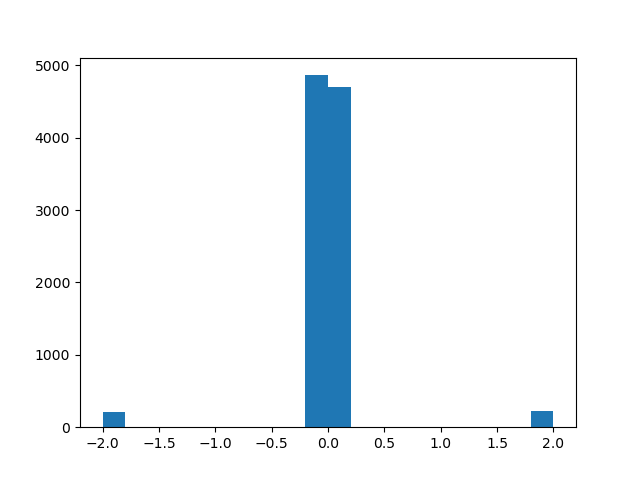
\includegraphics[scale=0.5]{subsurface_errors}
		\caption{Reconstruction Error}
		\label{fig:rec_error}
	\end{subfigure}\begin{subfigure}[t]{0.5\textwidth}
		\centering
		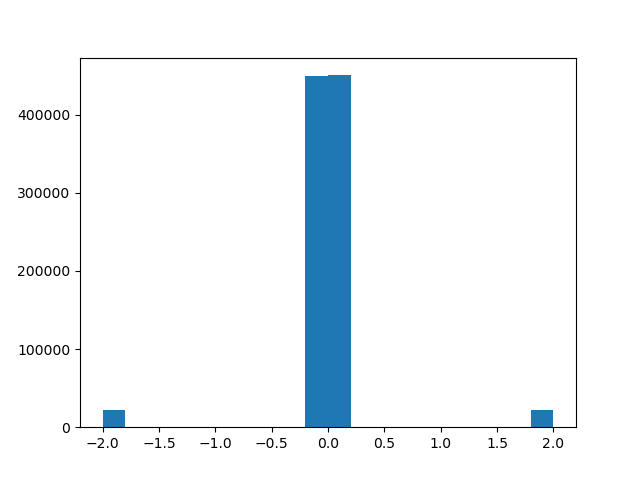
\includegraphics[scale=0.5]{subsurface_mixture_dist}
		\caption{Mixture distribution}
		\label{fig:mixture_dist}
	\end{subfigure}	
	\caption[Better modeling of the reconstruction error on the Subsurface dataset]{Left: Histogram of the reconstruction error of the UNetResPAC model on 100 generated images, with $\lambda = 1$. As we can see, is either close to 0, -2 or 2. Right:  Histogram of a million points sampled of a better fitting mixture distribution with two components: a Gaussian ($\mathcal{N}(\mu=0,\sigma=0.01)$) with a weight of 0.95 and a Beta distribution ($B(\alpha=\beta=0.05)$) with weight 0.05, which roughly corresponds to the error rate of the UNetResPAC model.}
\end{figure}

On the other hand, applying the developed approach to other applications or signals such as audio inpainting \citep{Marafioti2018} could also be an interesting perspective. Domains in which measuring points in any signal is costly or very noisy could benefit from an approach that allows fast sampling of potential solutions.
